\section{Evaluation}

\subsection{Source Code Classification}
\subsubsection{Data Set}
To evaluate wether \textbf{Code-RNN} is sufficient to extract method's function information, we apply \textbf{Code-RNN} to the function classify problem of methods. For classification, there are no existing data set for us to use, so we conduct a new methods set from Google Code Jam contest (2008$\sim$2016).

In one contest, all solutions of one problem have the same function, so if we can classify all methods to its own problem correctly we can say that our model \textbf{Code-RNN} is sufficient and meaningful.

We downloaded totally 120353 Java solutions in Google Code Jam from 2008 to 2016 and select 12 problems' solutions from them.\footnote{All solutions are freely available on the web http://www.go-hero.net/jam/16.} Then we choose six problems' solutions as training set(10724 methods)
%(6648+1997+2079=10724 methods)
 and the other 6 problems' solutions as test set(30 methods)
%(723 methods)
. The information of training set and test set is shown in Table \ref{table:method_data}.


\renewcommand{\multirowsetup}{\centering}
\begin{table}[!htb]
\centering
\caption{Data Set}
\label{table:method_data}
\begin{tabular}{|c|c|c|c|}
 \hline
  & problem name & year &\# of methods  \\
 \hline
 \multirow{6}{1.5cm}{Training Set} & Cookie Clicker Alpha & 2014 &%1008 301 330
 1639\\
 \cline{2-3}
  & Counting Sheep & 2016 &%1091 310  321
  1722\\
 \cline{2-3}
  & Magic Trick & 2014 &%1383 419 432
  2234\\
 \cline{2-3}
 & Revenge of the Pancakes & 2016 &%740 234 240
 1214\\
 \cline{2-3}
 & Speaking in Tongues & 2012 &%1064 316 309
 1689\\
 \cline{2-3}
 & Standing Ovation & 2015 &%1362 417 447
 2226\\
 \hline
 \multirow{6}{1.5cm}{Test Set} & All Your Base & 2009 & 5 \\ %&122\\
 \cline{2-3}
 & Consonants & 2013 & 5 \\ %&123\\
 \cline{2-3}
 & Dijkstra & 2015 & 5 \\ %&120\\
 \cline{2-3}
 & GoroSort & 2011 & 5 \\%&129\\
 \cline{2-3}
 & Osmos & 2013 & 5 \\ %&126\\
 \cline{2-3}
 & Part Elf & 2014 & 5 \\ %&103\\
 \hline
\end{tabular}
\end{table}

\subsubsection{Training}

Our Code-RNN model is just a method representation model, to achieve the goal of classifying methods, we apply the softmax function to the output of Code-RNN and calculate the loss with labels to train our model Code-RNN. To gain a better result we also use AdaGrad method~\cite{duchi2011adaptive} to apply unique learning rate to every parameter.

\subsubsection{Label Methods}

Because the problems in test set are not seen in the training set, we need to determine the label of every problem in test set firstly after classifying test set.
Then we can calculate accuracy, F1 score and so on.

We list all possible combinations of labels and use accuracy as the measurement standard to choose the largest accuracy label combination as the final label. The accuracies of final label in different models are shown in TABLE \ref{table:accuracy}. We can see that the accuracy of Code-RNN Average model is the largest one.

\begin{table}[!htb]
\centering
\caption{Accuracy of Final Label}
\label{table:accuracy}
\begin{tabular}{|c|c|c|c|c|}
 \hline
 Model & Accuracy  \\
 \hline
 Language Embedding Average & 0.3667\\
 \hline
 Language Embedding Sum & 0.3667 \\
 \hline
 Code-RNN Average & \textbf{0.5} \\
 \hline
 Code-RNN Sum & 0.4333 \\
 \hline
 inter node Code-RNN Average & 0.4667 \\
 \hline
 inter node Code-RNN Sum & 0.4667 \\
 \hline
\end{tabular}
\end{table}

\subsubsection{Result}

\begin{enumerate}[(i)]

\item Rename

We also rename all the identifiers' name to simple character such as `a', `b' and `c' in the test set. For example, after renaming, the code snippet in Fig. \ref{fig:code_rnn} will be below.
\begin{lstlisting}
  if (!a){
    b = false;
  }
  if (b){
    return true;
  }
\end{lstlisting}

 Then calculate the purity and F1 score both in rename test set and original test set. These values are in the TABLE \ref{table:purity}. Again the Code-RNN Average model is the largest one of all.

 From TABLE \ref{table:purity}, after renaming the result of Code-RNN become worse, so the identifiers' names are very useful in our model Code-RNN.

\begin{table}[!htb]
\centering
\caption{Purity and Average F1}
\label{table:purity}
\begin{tabular}{|c|c|c|c|c|c|}
 \hline
 & Purity  & Purity  & F1  & F1  \\ %& All\\
 &  original &  rename &  original &  rename \\
 \hline
 Language Embedding Average & 0.400 & 0.433 & 0.3515 & 0.3492 \\% & \textbf{0.3734}\\
 \hline
 Language Embedding Sum & 0.3667 & 0.4333& 0.2846 & 0.3288 \\%& 0.3582\\
 \hline
 Code-RNN Average & \textbf{0.533} & \textbf{0.500} & \textbf{0.4774} & \textbf{0.4462} \\% & 0.3513\\
 \hline
 Code-RNN Sum & 0.4667 & 0.3667 & 0.3945 & 0.2951\\% & 0.3610\\
 \hline
 inter node Code-RNN Average & 0.4667 & 0.4667 & 0.4167 & 0.4167 \\%& 0.3555\\
 \hline
 inter node Code-RNN Sum & 0.4667 & 0.4667 & 0.4187 & 0.4187 \\%& 0.3568\\
 \hline
\end{tabular}
\end{table}


\item F1 score

F1 values in TABLE~\ref{table:purity} are the average F1 values of test set's six problems.
TABLE \ref{table:F1_30} shows the F1 scores for every problem and we can see that Language Embedding model doesn't have any largest value while Code-RNN Average model has three largest value. This is because Code-RNN Average contains both of structure information and natural words information. And \textbf{Average} model guarantees no mater how many children one node has, order of magnitude of representation vector would be same as the parent's own vector, so that the contribution of parent and children can be considered equally.

Above all, the Code-RNN Average model is the best one and we choose this model to generate comment for methods.

%\begin{table*}[!htb]
%\centering
%\caption{F1 score}
%\label{table:F1_30}
%\begin{tabular}{|c|c|c|c|c|c|c|c|}
% \hline
% problem name& Dijkstra & Part Elf & All Your Base & GoroSort & Consonants & Osmos & average F1\\
% \hline
% Language Embedding Average & 0.3333 & 0.4286 & 0.3636 & 0.4 & 0.3333 & 0.25 & 0.3515 \\
% \hline
% Language Embedding Sum & 0.5333 & 0.3333 & 0.3077 & 0 & 0.5333 & 0 & 0.2846 \\
% \hline
% Code-RNN Average & 0.5714 & 0.6667 & 0.5 & 0 & \textbf{0.6} & \textbf{0.5263} & \textbf{0.4774}\\
% \hline
% Code-RNN Sum & 0.5455 & \textbf{0.7273} & 0.4444 & 0.25 & 0 & 0.4 & 0.3945\\
% \hline
% inter node Code-RNN Average & 0.5 & 0.6 & \textbf{0.5556} & \textbf{0.4444} & 0 & 0.4000 & 0.4167\\
% \hline
% inter node Code-RNN Sum & \textbf{0.6667} & 0.6154 & 0 & \textbf{0.4444} & 0.2857 & 0.5 & 0.4187 \\
% \hline
%\end{tabular}
%\end{table*}


\begin{table}[!htb]
\centering
\caption{F1 score}
\label{table:F1_30}
\begin{tabular}{|p{0.15\columnwidth}|p{0.07\columnwidth}|p{0.06\columnwidth}|p{0.06\columnwidth}|p{0.1\columnwidth}|p{0.11\columnwidth}|p{0.07\columnwidth}|p{0.07\columnwidth}|}
 \hline
 problem name&Dijkstra&Part Elf&All Your Base&GoroSort&Consonants&Osmos&average F1\\
 \hline
 Language Embedding Average & 0.33 & 0.43 & 0.36 & 0.40 & 0.33 & 0.25 & 0.35 \\
 %Average & & & & & & &\\
 \hline
 Language Embedding Sum & 0.53 & 0.33 & 0.31 & 0 & 0.53 & 0 & 0.28 \\
 \hline
 Code-RNN Average & 0.57 & 0.67 & 0.5 & 0 & \textbf{0.6} & \textbf{0.53} & \textbf{0.48}\\
 \hline
 Code-RNN Sum & 0.55 & \textbf{0.73} & 0.44 & 0.25 & 0 & 0.4 & 0.39\\
 \hline
 inter node Code-RNN Average & 0.5 & 0.6 & \textbf{0.56} & \textbf{0.44} & 0 & 0.40 & 0.42\\
 \hline
 inter node Code-RNN Sum & \textbf{0.67} & 0.62 & 0 & \textbf{0.44} & 0.29 & 0.5 & 0.42 \\
 \hline
\end{tabular}
\end{table}


%\begin{table*}[!htb]
%\centering
%\caption{F1 score}
%\label{table:F1}
%\begin{tabular}{|c|c|c|c|c|c|c|}
% \hline
% problem name& Dijkstra & Part Elf & All Your Base & GoroSort & Consonants & Osmos \\
% \hline
% bag of words average & 0.3929 & 0 & 0.4215 & \textbf{0.4829} & 0.2905 & 0.3668 \\
% \hline
% bag of words sum & 0.3795 & 0.0154 & \textbf{0.4911} & 0.5 & 0 & 0.2759  \\
% \hline
% tree average & 0.3778 & \textbf{0.4731} & 0.25 & 0.0552 & 0.3056 & \textbf{0.4127} \\
% \hline
% tree sum & 0.2890 & 0.2276 & 0.4075 & 0.4622 & 0.1437 & 0.3274 \\
% \hline
% inter node average & 0.3878 & 0.4641 & 0.4353 & 0.0156 & 0.1279 & 0.3542\\
% \hline
% inter node sum & \textbf{0.4223} & 0.5149 & 0 & 0.0859 & \textbf{0.4207} & 0.2710 \\
% \hline
%\end{tabular}
%\end{table*}

\end{enumerate}



\subsection{Generation Model}
\subsubsection{Data Set}
We downloaded seven open-source Java code repositories from GitHub,
and their information is showed in Table \ref{table:repos}.  Then we
select all commented methods in the repository except for the constructor methods of every class because the functions of all constructor methods are same, to construct the classes. And commented methods have original comments wrote by developers so that we can use them as ground truth to train and test.

\begin{table*}[!htb]
\centering
\scriptsize{
\caption{\label{table:repos} Repositories Information}
\centering
\begin{tabular}{|c|c|c|c|c|c|}
\hline
Project & Description & \# of bytes & \# of Java Files& \# of Methods& \# of Commented Methods\\
%&  & bytes & Files & Methods & comments \\
\hline
%& & & & & \\
guice & a lightweight dependency injection framework for Java 6 and above. & 89M & 528 & 3261 & 397 \\
%& & & & & \\
\hline
%& & & & & \\
jna & provides Java programs easy access to native shared libraries  & 294M & 304 & 2254 & 475 \\

%& & & & & \\
\hline
%& & & & & \\
zxing & a multi-format 1D/2D barcode image processing library implemented in Java & 373M & 471 & 2294 & 321 \\
%& & & & & \\
\hline
%& & & & & \\
%libgdx & a cross-platform Java game development framework based on OpenGL (ES)& 989M & 1906 & 18889 & 2828 \\
%& & & & & \\
%\hline
%& & & & & \\
cocos2d & cocos2d for android, based on cocos2d-android-0.82 & 78M & 512 & 3677 & 1182 \\
%& & & & & \\
\hline
%& & & & & \\
%spring-security & provides security services for the Spring IO Platform. & 42M & 1449 & 6336 & 983 \\
%& & & & & \\
%\hline
%& & & & & \\
%& The Guava project contains several of Google's  & & & & \\
%& core libraries that we rely on in our& & & & \\
%guava & Java-based projects: collections, caching, primitives & 80M & 1710 & 20321 & 3079 \\
%&  support, concurrency libraries, common annotations, & & & & \\
%& string processing, I/O, and so forth. & & & & \\
%& & & & & \\
%\hline
%& & & & & \\
rhino & a Java implementation of JavaScript.& 21M & 352 & 4610 & 1195 \\
%& & & & & \\
\hline
%& & & & & \\
mockito & Tasty mocking framework for unit tests in Java & 80M & 916 & 4439 & 511 \\
%& & & & & \\
\hline
%& & & & & \\
jersey & a REST framework that provides JAX-RS Reference Implementation and more. & 73M & 2743 & 14374 & 2540\\
%& & & & & \\
\hline
%& & & & & \\
%elasticsearch & Elasticsearch is a distributed RESTful search engine & 142M & 3978 & 24572 & 7109 \\
%& built for the cloud. & & & & \\
%& & & & & \\
%\hline
%& & & & & \\
%neo4j & the world��s leading Graph Database. & 270M & 4125 & 24529 & 1197\\
%& & & & & \\
%\hline
\end{tabular}
}
\end{table*}

%\subsubsection{Call Graph}
%
%I also need to try different depth of call graph, no only without invocation.

\subsubsection{Big Project}

How to handle big project.

\subsubsection{Sequence-to-Sequence Model}

Sequence-to-Sequence model is a popular model based on Recurrent Neural Network, it is used widely in Machine Translation \cite{sutskever2014sequence}\cite{bahdanau2014neural}, Conversation \cite{vinyals2015neural}, Summarization \cite{nallapati2016abstractive}\cite{nallapati2016text}, Image Caption \cite{xu2015show} and so on.

A basic sequence-to-sequence model, as introduced in Cho et al.\cite{cho2014learning}, consists of two recurrent neural networks (RNNs): an encoder that processes the input and a decoder that generates the output. It's structure is showed in Fig. \ref{fig:seq2seq}.

\begin{figure}[!htb]
\centering
	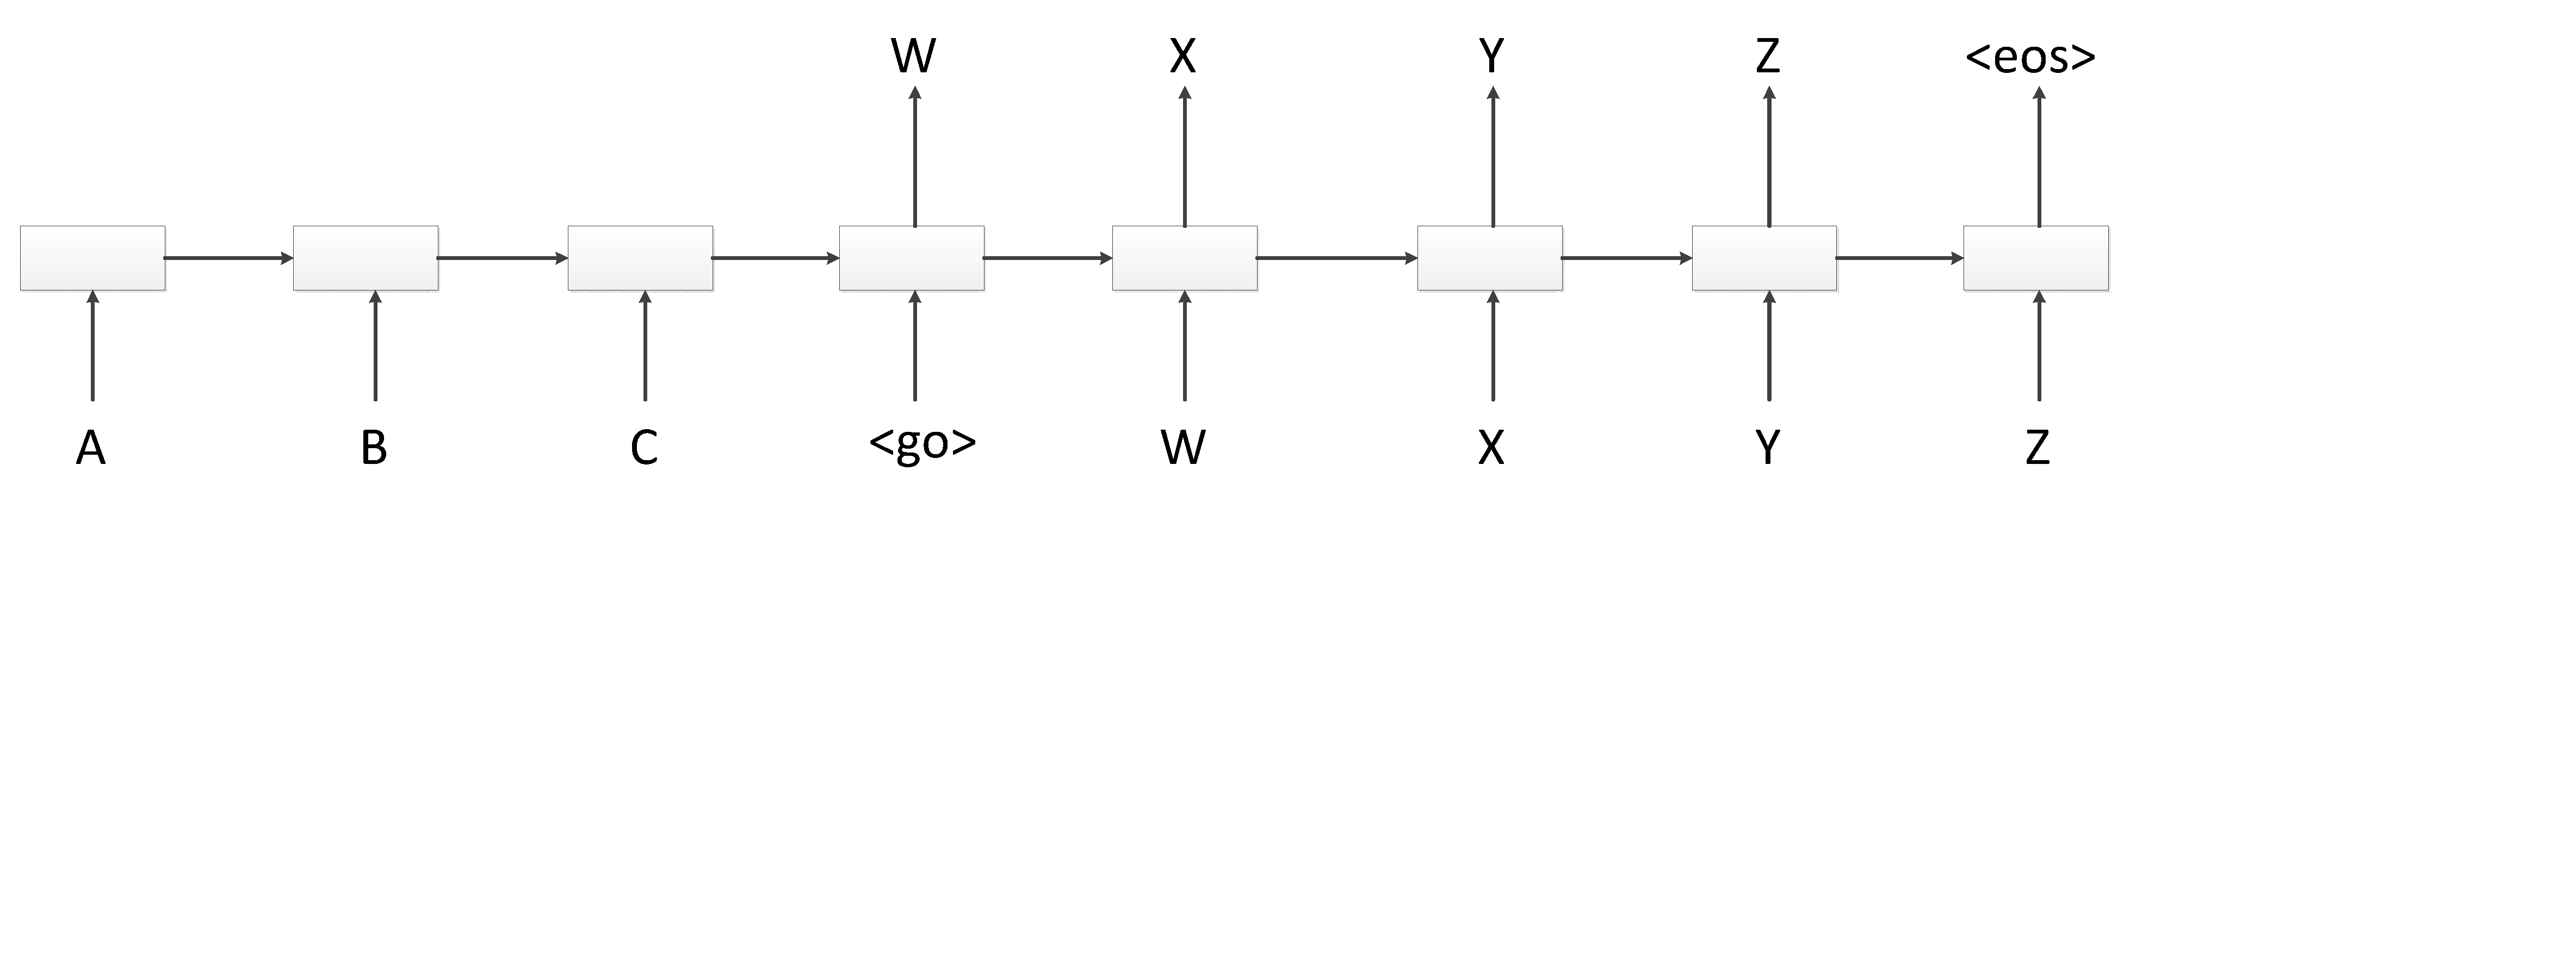
\includegraphics[width=\linewidth]{img/seq2seq.pdf}
\caption{Basic Seq2Seq architecture}\label{fig:seq2seq}
\end{figure}

In the basic model depicted above, every input has to be encoded into a fixed-size state vector, as that is the only thing passed to the decoder. To allow the decoder more direct access to the input, an attention mechanism was introduced in Bahdanau et al.\cite{bahdanau2014neural}. The Sequence-to-Sequence model we used here contains the attention mechanism.

To use Sequence-to-Sequence model, our input and output must be two sequences. For our source code comments generation problem, the output is comments and it is naturally sequences. So we must translate the input source code into a sequence first. According to translating methods, we have two kinds of Sequence-to-Sequence model as baseline in our paper. Next, we will discuss more details of these two methods.

\begin{enumerate}[(i)]

\item Natural Word Sequence

In this methods,we delete all special symbols (``\$'', ``('', ``+'', $\cdots$) in the source codes and split all the long forms to multiple words. We also change all characters into lower-case. Finally we put these words in a sequence and sorted by their existing order in the source code.

The natural word sequence of the code snippet in Fig. \ref{fig:code_rnn} is:
\textbf{if, found, all, found, false, if, all, found, return, true.}

We call this model \textbf{Text Seq2Seq}.

\item Parse Tree Sequence

In this methods, we construct the parse tree of methods firstly, the parse tree is like the Code-RNN in Fig. \ref{fig:code_rnn}. Then we use the pre-ordered traversal sequence of parse tree as the input of Sequence-to-Sequence model. Fig. \ref{fig:tree_sequence} shows the pre-ordered traversal sequence of the parse tree in Fig. \ref{fig:code_rnn}. Comparing with Natural Word Sequence, this sequence also contains some structure information, for example, ``IfStatement' and ``ThenStmt''.

Q. Chen et al.~\cite{chen2016enhancing} also use the pre-ordered traversal sequence of tree as a input sequence of model for natural language inference, but its tree is binary tree but our tree is arbitrarily tree.

We call this model \textbf{Tree Seq2Seq}.

\begin{figure*}[!htb]
\centering
\noindent\rule[0.25\baselineskip]{\textwidth}{1pt}

\begin{minipage}{0.9\linewidth}

root, IfStatement, ......, IfStatement, IfToken, if, OpenParenToken, (, Condition, NameExpr, CombineName, all, found, CloseParaenToken, ), ThenStmt, BlockStmt, BlockBeginToken, \{, ReturnStmt, ReturnToken, return, BooleanLiteralExpr, true, BlockEndToken, \}
\end{minipage}

\noindent\rule[0.25\baselineskip]{\textwidth}{1pt}

\caption{Parse Tree Sequence}\label{fig:tree_sequence}
\end{figure*}

\end{enumerate}

After generating input data, we use the code that wrote by D. Britz et al.~\cite{Britz:2017} to run sequence-to-sequence model as baseline.\footnote{This code can be downloaded from https://github.com/google/seq2seq.}


\subsubsection{Rouge Value}

To evaluate comment generation model, we choose the Rouge model\cite{lin2004rouge}. Rouge has been used in many summary works\cite{donahue2015long} \cite{haghighi2009exploring} \cite{rush2015neural}
 as measurement standard. For Rouge model, there are many methods to calculate score, we choose Rouge-2 value in this paper.

We firstly use Text Seq2Seq, Tree Seq2Seq and Code-RNN these three model to train within the seven repositories. For one project, we choose part of their commented methods as training set and the other methods as text set. The results of within repository are listed in Table \ref{table:rouge}.

For most of repositories, Tree Seq2Seq model is better than Text Seq2Seq model because it contains some structure information and our model Code-RNN is better than both Seq2Seq models. Because our model maintain the structure information and embed it into neural network not like the Tree Seq2Seq just use the pre-ordered traversal
sequence of parse tree.

Then we evaluate Code-RNN cross repositories. For example, we train our model on the repository ``zxing'' and use the trained parameter to generate comments for the commented methods in repository ``guice''. The results are listed in
Table \ref{table:cross_rouge}.

Every row in Table \ref{table:cross_rouge} shows the Rouge-2 value of the same repository that tested by different parameters. For example, we train the model on different repositories and test them on project ``zxing'' then put values in the first row. We also highlight the largest value in every row. We can see that the model trained by ``jan'' and ``mockito'' are the best, and they are also the largest two in Table \ref{table:rouge}. And the Rouge-2 value of repository ``cocos2d'' train by ``jna'' and ``mockito'' even better than the value that trained by itself.


\begin{figure}[!htb]
\centering
	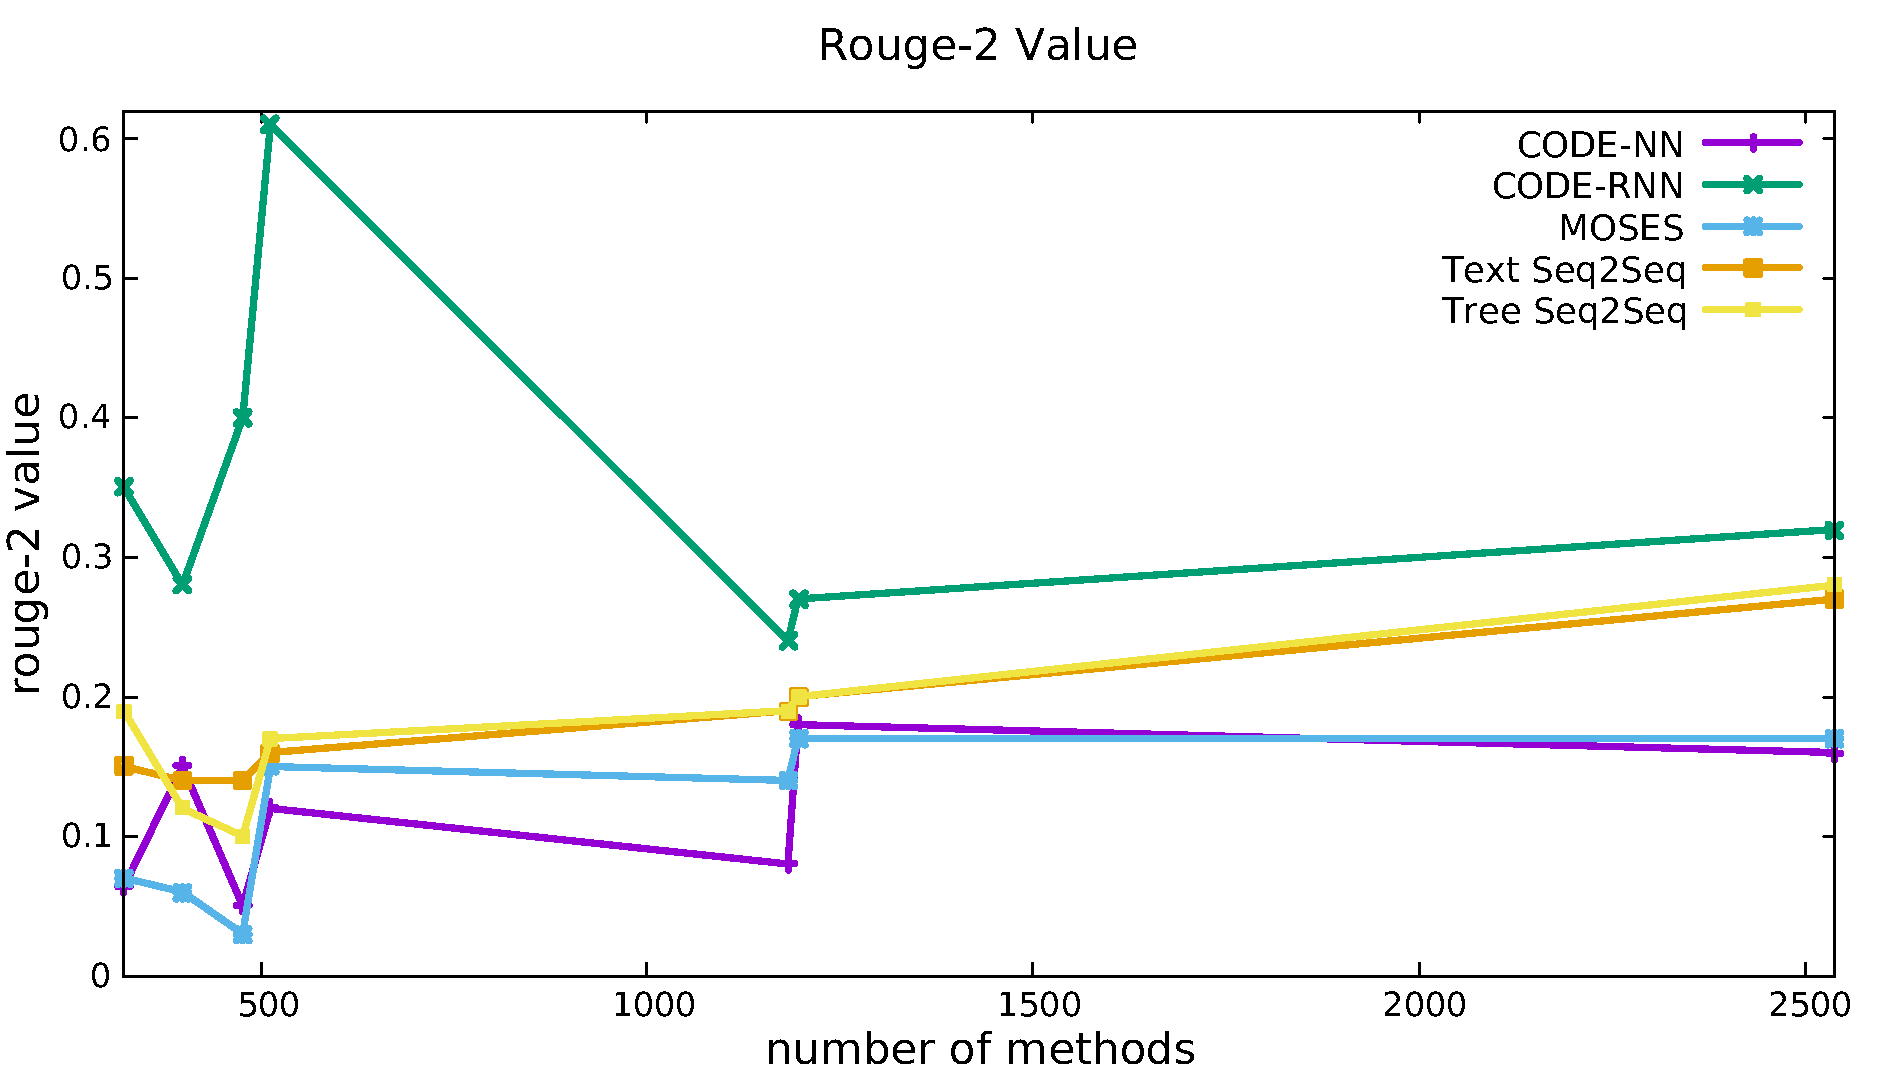
\includegraphics[width=\linewidth]{img/rouge_2_img.pdf}
\caption{Rouge-2 Value Figure}\label{fig:rouge_img}
\end{figure}



%\begin{table*}[th]
%\caption{Rouge-2 Values within Repository}
%\center
%{
% \begin{tabular}{|c|c|c|c|c|c|c|c|c|c|c|c|c|}
% \hline
%  Repo Name& zxing & jersey & guice & cocos2d & jna & rhino & mockito\\
% \hline
%% call graph depth & \color{red}{1} & \color{red}{1} & \color{red}{1}  &\color{red}{1} & \color{red}{1} & \color{red}{1} & \color{red}{1}\\
%% \hline
%Text Seq2Seq
%& 0.14972 & 0.268125 & 0.140236 &  0.193651 & 0.142333 & 0.19639 & 0.16166 \\
%\hline
%Tree Seq2Seq
%& 0.192659 &  0.278576 & 0.120983 & 0.194555 & 0.102747 & 0.198959 & 0.172287\\
%\hline
%MOSES
%& 0.07437 & 0.16851 & 0.05812 & 0.14305 & 0.06295 & 0.17240 & 0.14940\\
%\hline
%Code-NN(100)
%& 0.05488 & 0.07244 & 0.03325 & 0.05388 & 0.04462 & 0.10514 & 0.05965 \\
%\hline
% Code-RNN
%& 0.35172 &  0.32093 & 0.27626 &  0.24320 & 0.40093 & 0.26793 & 0.61043\\
%\hline
%% ROUGE-3
%%& 0.25448 & 0.25061 & 0.18166 & 0.14968 & 0.28420 & 0.17943 & 0.51536\\
%% \hline
%%  ROUGE-4
%%& 0.16341 & 0.19946 & 0.13349 & 0.09462 & 0.20482 & 0.12228 & 0.44240 \\
%% \hline
%% ROUGE-L
%%& 0.54497 & 0.44609 & 0.44232 & 0.43974 & 0.57992 & 0.43533 & 0.73452\\
%% \hline
%%  ROUGE-S*
%%& 0.32324 & 0.27854 & 0.26267 & 0.22013 & 0.36437 & 0.22310 & 0.57267\\
%% \hline
%%  ROUGE-SU*
%%& 0.34894 & 0.30012 & 0.28717 & 0.25157 & 0.39823 & 0.25341 & 0.59412\\
%% \hline
% \end{tabular}
% }
%
%\label{table:rouge}
%\end{table*}


\begin{table}[th]
\caption{Rouge-2 Values within Repository}
\center
{
 \begin{tabular}{|c|c|c|c|c|c|c|c|c|c|c|c|c|}
 \hline
  Repo Name& zxing & jersey & guice & cocos2d & jna & rhino & mockito\\
 \hline
Text Seq2Seq
& 0.13 & 0.22 & 0.10 &  0.18 & 0.14 & 0.18 & 0.14 \\
\hline
Tree Seq2Seq
& \color{red}{0.19} &  0.23 & 0.09 & 0.14 & 0.9 & 0.19 & 0.17\\
\hline
MOSES
& 0.07 & 0.17 & 0.06 & 0.14 & 0.06 & 0.17 & 0.15\\
\hline
Code-NN(100)
& 0.064 & 0.15 & 0.05 & 0.12 & 0.08 & 0.18 & 0.16 \\
\hline
 Code-RNN
& \textbf{0.35} & \textbf{0.32} & \textbf{0.28} &  \textbf{0.24} & \textbf{0.40} & \textbf{0.27} & \textbf{0.61}\\
\hline
Code-RNN(cross)
& 0.09 & 0.13 & 0.09 &  0.19 & 0.25 & 0.18 & 0.26\\
\hline
 \end{tabular}
 }

\label{table:rouge}
\end{table}


%\begin{table*}[th]
%\caption{Rouge-2 Values cross Repositories}
%\center
% \begin{tabular}{|c|c|c|c|c|c|c|c|c|}
% \hline
%  \diagbox{Eval}{Train} & zxing & guice & jna & rhino & jersey & cocos2d &mockito \\
% \hline
% zxing
%& * & 0.05886 & \textbf{0.21251} & 0.15398 & 0.07264 & 0.18783 & 0.19416 \\
%\hline
% guice
%& 0.08126 & * & 0.22590 & 0.20599 & 0.18897 & 0.20374 & \textbf{0.31475} \\
% \hline
%  jna
%& 0.08497 & 0.0884 & * & 0.15991 & 0.13076 & 0.14773 & \textbf{0.26046} \\
% \hline
% rhino
%& 0.07490 & 0.09192 & 0.23922 & * & 0.12816 & 0.17878 & \textbf{0.26196} \\
% \hline
%  jersey
%& 0.10201 & 0.09565 & 0.25253 & 0.18636 & * & 0.19703 & \textbf{0.27913} \\
% \hline
%  cocos2d
%& 0.09273 & 0.08466 & \textbf{0.28518} & 0.17720 & 0.10072 & * & 0.24975 \\
% \hline
% mockito
%& 0.10840 & 0.12796 & \textbf{0.27933} & 0.20330 & 0.14402 & 0.19551 & * \\
% \hline
% \end{tabular}
%\label{table:cross_rouge}
%\end{table*}

\begin{table}[th]
\caption{Rouge-2 Values cross Repositories}
\center
 \begin{tabular}{|c|c|c|c|c|c|c|c|c|}
 \hline
  \diagbox{Eval}{Train} & zxing & guice & jna & rhino & jersey & cocos2d &mockito \\
 \hline
 zxing
& * & 0.06 & \textbf{0.21} & 0.15 & 0.07 & 0.19 & 0.19 \\
\hline
 guice
& 0.08 & * & 0.23 & 0.21 & 0.19 & 0.20 & \textbf{0.31} \\
 \hline
  jna
& 0.08 & 0.09 & * & 0.16 & 0.13 & 0.15 & \textbf{0.26} \\
 \hline
 rhino
& 0.07 & 0.09 & 0.24 & * & 0.13 & 0.18 & \textbf{0.26} \\
 \hline
  jersey
& 0.10 & 0.10 & 0.25 & 0.19 & * & 0.20 & \textbf{0.28} \\
 \hline
  cocos2d
& 0.09 & 0.08 & \textbf{0.29} & 0.18 & 0.10 & * & 0.25 \\
 \hline
 mockito
& 0.11 & 0.13 & \textbf{0.28} & 0.20 & 0.14 & 0.20 & * \\
 \hline
 \end{tabular}
\label{table:cross_rouge}
\end{table}



\subsubsection{Comment Example}

We put three comment examples in Fig. \ref{fig:comment_example}. Because we delete all punctuation, the comments listed here are lack of the punctuation. However, we can see that the comments generated by our model are readable and meaningful. We also write the project name that the method comes from in the figure, for example, the first method belongs to project jna.

For the first example, our model use the word ``mapped'' to replace the word ``dispatch'' in the comment, and these two words have the similar meaning. The situation of replacing words also appears in the third example. ``sets the parent of the {\color{red}{new}} statement'' in the original comment while ``sets the parent of the {\color{red}{declaration}} statement'' in the generated comment by our model. Our comment specify the kind of statement not just the ``new statement'' in the original comment.

In the second example, comparing with the original comment our model's generated comment maintain the most important part ``the number of vertices''.

However, the comments generated by our model has one problem is that the front part is quite different with the original comments while the latter part almost the same as original comments. The third example also has this problem. This may because we feed the method vector at every step and after some steps the influence of method vector is big enough to generate the correct comments. So we can highlight the influence or weight of method vector at the beginning steps of Recurrent Neural Network to improve our model in the future work.

\KZ{The last fig didn't show up in my pdf!}
\begin{figure}[th]
%\begin{minipage}{\linewidth}
%\begin{tabular}{|c|p{0.48\columnwidth}|}
% \hline
%   \color{red}{original comment} & gets the i dispatch pointer\\
% \hline
%   \color{green}{generated comment} & checks gets the i mapped pointer\\
% \hline
% \end{tabular}
%\\[0cm]
%\begin{lstlisting}
% Project: jna
% public PointerByReference getIDispatchPointer() {
%        return pDispatch;
%    }
%\end{lstlisting}
%\end{minipage}
%%com.sun.jna.platform.win32.COM.COMBindingBaseObject.getIDispatchPointer
%%\\[1cm]
%\vfill

\begin{minipage}{\linewidth}
\begin{tabular}{|c|p{0.48\columnwidth}|}
 \hline
   \color{red}{original comment} & return the number of vertices\\
 \hline
   \color{green}{generated comment} & info and the number of vertices\\
 \hline
 \end{tabular}
\\[0cm]
\begin{lstlisting}
 Project: cocos2d
  public int getVertexCount() {
        return vertices.size();
    }
\end{lstlisting}
\end{minipage}
%org.jbox2d.collision.PolygonDef.getVertexCount
%\\[1cm]
\vfill

\begin{minipage}{\linewidth}
\begin{tabular}{|c|p{0.48\columnwidth}|}
 \hline
   \color{red}{original comment} & adds a statement to the end of the statement list sets the parent of the new statement to this node updates its start offset to be relative to this node and sets the length of this node to include the new child\\
 \hline
   \color{green}{generated comment} & no this generation to the end of the statement list sets the parent of the declaration statement to this node updates its start offset to be relative to this node and sets the length of this node to include the new child\\
 \hline
 \end{tabular}
%\\[0cm]
\begin{lstlisting}
 project: rhino
 public void addStatement(AstNode statement) {
        assertNotNull(statement);
        if (statements == null) {
            statements = new ArrayList<AstNode>();
        }
        int end = statement.getPosition() + statement.getLength();
        this.setLength(end - this.getPosition());
        statements.add(statement);
        statement.setParent(this);
    }

\end{lstlisting}
\end{minipage}
%org.mozilla.javascript.ast.SwitchCase.addStatement
%\\[1cm]
\vfill

\begin{minipage}{\linewidth}
\begin{tabular}{|c|p{0.48\columnwidth}|}
 \hline
   \color{red}{original comment} & pushes a new type onto the output frame stack\\
 \hline
   \color{green}{generated comment} & todo pushes a new type onto the output frame stack\\
 \hline
 \end{tabular}
\\[0cm]
\begin{lstlisting}
 project: mockito
 private void push(final int type) {
        // creates and/or resizes the output stack array if necessary
        if (outputStack == null) {
            outputStack = new int[10];
        }
        int n = outputStack.length;
        if (outputStackTop >= n) {
            int[] t = new int[Math.max(outputStackTop + 1, 2 * n)];
            System.arraycopy(outputStack, 0, t, 0, n);
            outputStack = t;
        }
        // pushes the type on the output stack
        outputStack[outputStackTop++] = type;
        // updates the maximun height reached by the output stack, if needed
        int top = owner.inputStackTop + outputStackTop;
        if (top > owner.outputStackMax) {
            owner.outputStackMax = top;
        }
    }
\end{lstlisting}
% org.mockito.asm.tree.analysis.Frame.push
\end{minipage}

%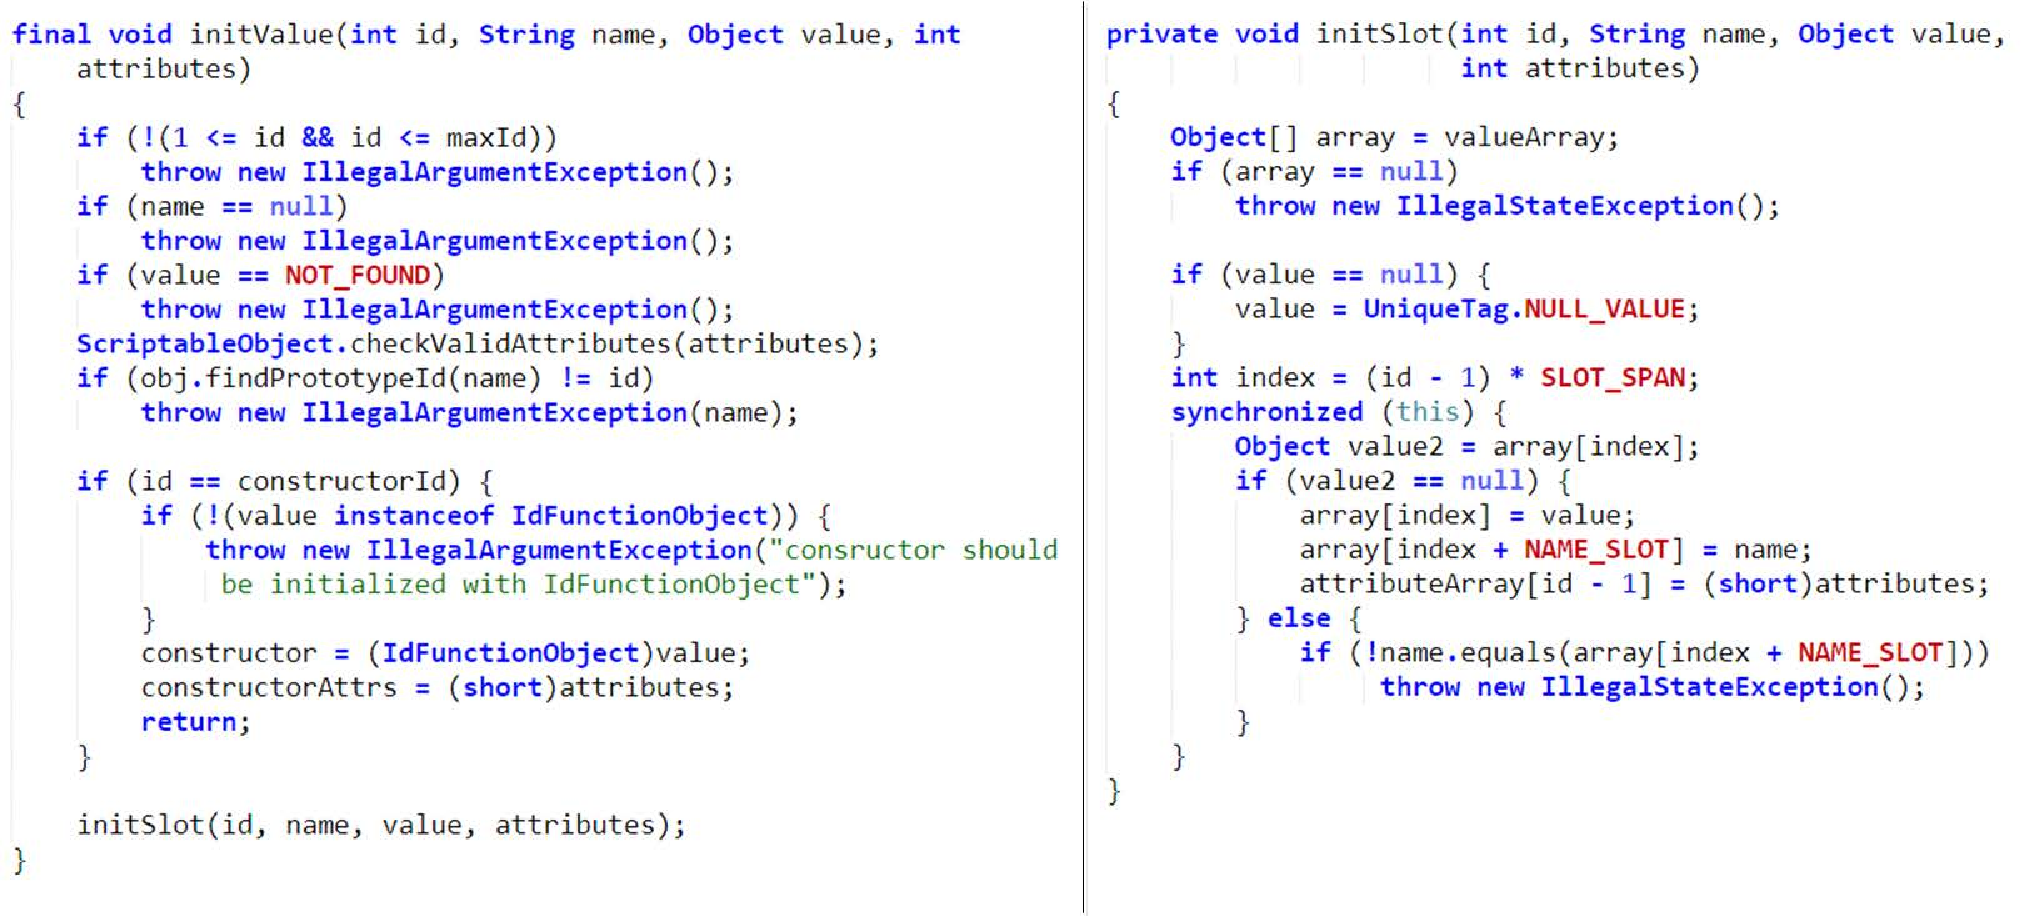
\includegraphics[width=16cm]{img/codeExample.pdf}
\caption{comment example}\label{fig:comment_example}
\end{figure}









